\documentclass{article}
\usepackage[utf8]{inputenc}

\title{Chem-131C-Lec6}

\author{swflynn }
\date{April 2017}

\usepackage{natbib}
\usepackage{graphicx}
\usepackage{braket}
\usepackage{amsmath}
\usepackage[margin=0.7in]{geometry}
\usepackage{subfigure}
\usepackage{tikz}
\usepackage{float}

\begin{document}

\maketitle

\section*{Lecture 6; 4/14/17}
Last lecture we started to look into the topic of thermodynamics.
We talked about the internal energy (the thermodynamic energy) U. 
We know from conservation of energy, that the energy of an isolated system is constant.
We can write the first law of thermodynamics in terms of the total work (w) and the heat (q). 
\begin{equation}
    \Delta U = q+w
\end{equation}

For an ideal gas that is monoatomic, the internal energy is $\frac{3}{2}$nRT (not true for any other system!). 
Looking at this equation we see that the ideal gas has an internal energy that depends on T only 
U(T,V,...) $\xrightarrow{\text{I.G.}}$ U(T). 

For example we could consider the van der Walls EOS (very common in chemistry), which accounts for the attraction between molecules (a-parameter) and the volume of molecules (b-parameter).
\begin{equation}
    \left( {P + \frac{{an^2 }}{{V^2 }}} \right)\left( {V - nb} \right) = nRT
\end{equation}
For this type of system U is U(T,V).

\subsection*{Free Expansion of a Gas}
Consider a free expansion of an ideal gas in an adiabatic container. 
Physically you have a gas in a box with a partition down the middle, the gas fills one side, the other side is vacuum.
Then, the partition magically disappears.
Because the gas expands into vacuum there is nothing to get in the way of the atoms as they expand, therefore no work is done (it is expanding into nothing). 
$\Delta$U is 0 for this process, and if the gas is ideal, there will be no change in temperature during the expansion.

In reality (a real gas) there must be some potential energy between the atoms (and therefore internal energy). 
So a more 'realistic' picture could consider a van der walls gas with a Lennard-Jones potential. 
\begin{figure}[h!]
    \centering
    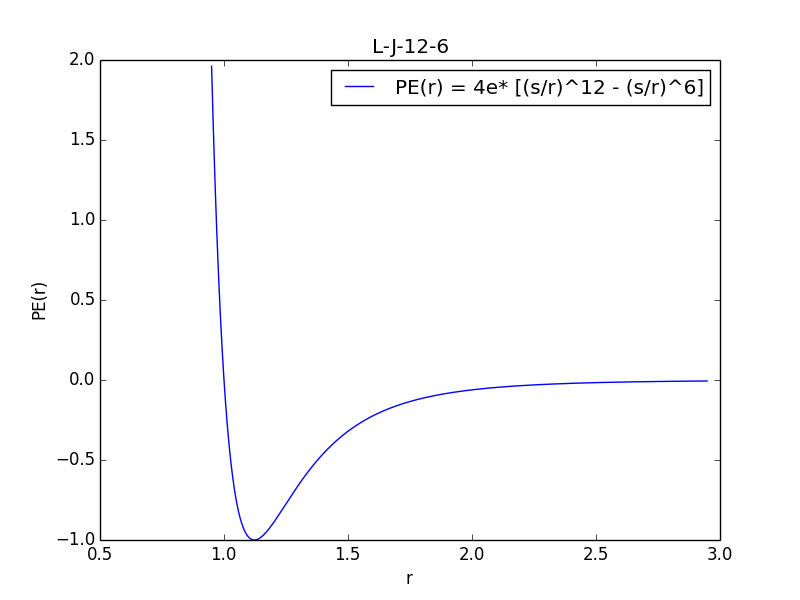
\includegraphics[width=0.9\textwidth]{L-J-12-6.png}
    \caption{Real Gas; L-J Potential Energy}
    \label{fig:LJ1}
\end{figure}
In a real system that is expanding, the potential energy will increase (r gets larger).
Conservation of energy still exists so our KE must decrease and therefore the Temperature decreases during the expansion of a real gas. 

\subsection*{Isothermal Compression and Expansion}
If a system is isothermal, it means that the temperature of the surroundings and system are equal. 
If the temperatures are equal then there is no $\Delta$T, if the gas is ideal then the internal energy would again be 0. 
If we compress a gas within a diathermal cylinder, heat transfer will (and does) occur. 
If we compress the gas, we are doing work on the gas, therefore the gas would have more energy. To keep the temperature the same heat must leave the system. 

\subsubsection*{Question}
Consider an isothermal compression of an ideal gas at T$_0$, P$_0$, and a compression from V$_0$ to $\frac{1}{2}$V$_0$. 
\begin{enumerate}
    \item What is the final temperature of the system?
    \item What is the final volume of the system. 
    \item What is the final pressure of the system
\end{enumerate}
By definition the temperature of the system can't change, therefore the final temperature is T$_0$. 
By construction we are cutting the volume in half, therefore the final volume is $\frac{V_0}{2}$. 
We are working with an ideal gas, so we can use the EOS to solve for the final pressure.
\begin{equation}
    \begin{split}
        P_0V_0=nRT, &\quad P_1V_1=nRT \\
        P_0V_0 &= P_1V_1 \\
        P_1 = \frac{2P_0V_0}{V_0} &= 2P_0
    \end{split}
\end{equation}
\subsubsection*{Compression Methods}
Consider now the method with which we compress the gas. 
We know that we must apply some external pressure on our cylinder to decrease the volume.
Intuition would tell you that the pressure you use would need to be greater than the pressure exerted by the gas. 
If we want to quickly compress the gas we should just push as hard as possible, if we are a little more patient we could ideally push with just a bit more force than the pressure of the gas. 
\begin{equation}
    \delta w = -FdV = -P_{ext}dV
\end{equation}
It is important to note here that we can intuitively understand it will take longer to compress the gas if we use a lower external pressure, however, thermodynamics itself never tells us anything about time. 
Remember, thermodynamics only considers systems in equilibrium, it says nothing about how long it takes to reach that equilibrium.
Questions about time enter the realm of chemical kinetics. 

How much work is done during this process? 
Assume that the external pressure is constant. 
\begin{equation}
\begin{split}
        \int \delta w = \int-P_{ext}dV \\
        w = -P_{ext}(V_2-V_1)
\end{split}
\end{equation}
If the system is an ideal gas in an isothermal container then q=-w.  

Now consider the \textbf{reversible} compression of a gas. 
The reversible limit is when your external pressure exactly matches (infinitesimally larger than) the pressure of the gas during every moment of the compression.
In this limit we can replace the external pressure with the pressure of the gas, and use an EOS for the gas instead; assume ideal:
\begin{equation}
\begin{split}
    P(V) &= \frac{nRT}{V} \\
    w_{r} &= -\int_{V1}^{V2} P(V)dV = -\int_{V1}^{V2} \frac{nRT}{V} dV \\
    w_{r} &= -nRT\ln \left[\frac{V_2}{V_1}\right]
\end{split}
\end{equation}
So let's compare a reversible and irreversible isothermal compression, assume ideal gas and compress the volume in half. 
\begin{center}
  \begin{tabular}{ | l | c |}
    \hline
    Irreversible & Reversible  \\ \hline
     w$_{ir}$= -P$_2$(V$_2$-V$_1$) & w$_r$= -nRT$\ln\frac{V_2}{V_1}$  \\ \hline
    =$\frac{-nRT}{V_2}(V_2-V_1)$ & =nRT$\ln\frac{V_1}{V_2}$  \\ \hline
    = nRT($\frac{V_1}{V_2}-1$) & =nRT $\ln\frac{V_1}{V_2}$ \\ \hline
    = nRT & =nRT ln(2)\\
    \hline
  \end{tabular}
\end{center}
From this simple analysis we see that the reversible work is less than the irreversible work. 
This should make intuitive sense, we do not waste any extra energy in doing the reversible compression, therefore our work is lower. 

When we compress a gas we are innately decreasing the entropy of the system, think of entropy as the available 'states' for the gas to occupy, with a smaller volume there are less conformations. 
Entropy can be written as 
\begin{equation}
\Delta S = \frac{q}{T}
\end{equation}
When we compress the gas heat must enter the environment, therefore the entropy of the environment must increase. 

Consider now compressing a gas irreversibly, we therefore do more work than optimal to get the compression. 
If we then let the gas expand, the amount of work we gain from this process is much less than what we had to put in for the compression, all we get is the gain in entropy of the environment. 

\subsection*{Heat Capacity}
The heat capacity C(T,V) is a state function. 
Consider the internal energy total differential.
\begin{equation}
dU = \left(\frac{\partial U}{\partial T}\right)_VdT + \left(\frac{\partial U}{\partial V}\right)_TdV
\end{equation}
The first term in this total differential is defined as the constant volume heat capacity
\begin{equation}
C_v(T) \equiv \left(\frac{\partial U}{\partial T}\right)_V
\end{equation}
Consider the ideal gas, the second term is 0 because the internal energy of a constant temperature system is 0. 

For a monoatomic ideal gas (at moderate temperature) it can be shown that. 
\begin{equation}
C_v(T) = \left(\frac{\partial U}{\partial T}\right)_V = \frac{3}{2}nR
\end{equation}
The diatomic replaces the coefficient with 5/2. 

With this formula we can evaluate the ideal gas heat capacity. 
\begin{equation}
C_v(T) = \left(\frac{\partial U}{\partial T}\right)_V = \frac{d}{dT} \frac{3}{2}nRT =  \frac{3}{2}nR
\end{equation}
Now take the definition of heat capacity and start assuming things!
\begin{equation}
C_v(T) \rightarrow C_v \quad \text{then} \quad \Delta U = C_v\Delta T
\end{equation}
This description gives a better intuition, it says heat capacity is simply the change in internal energy with temperature, meaning how much heat do you need to raise the temperature. 
Something with a high heat capacity stays warm for a very long time, if you have a small heat capacity you lose your heat quickly. 

\subsection*{Adiabatic Compression}
Finally let's consider an adiabatic compression of an ideal gas. 
By definition no heat can be exchanged between the system and surroundings. 
If we do work on the system (compress the gas) then the temperature of the gas must increase. 
If there is a temperature change then the internal energy will subsequently change, and will be equal to the work (first law). 


\section{Supplemental Notes}

\subsection*{Lennard-Jones Potential}
We know from general chemistry that a 'long-range' interaction between neutral non-bonded atoms is the van der Wall's interaction (aka London-Dispersion forces). 
When trying to model chemical systems, computational chemists developed a potential energy that accounts for these long-term interactions, called the Lennard-Jones Potential. 
It is a 2-body potential heavily used in molecular dynamics simulations. 
It is commonly used in combination with the van der Wall's equation to model real gases.
\begin{equation}
PE(r)=4 \epsilon \left[\left(\frac {\sigma}{r}\right)^{12}-\left(\frac {\sigma}{r}\right)^6\right]
\end{equation}
Where $\epsilon$ is the depth of your potential well, $\sigma$ is the distance (finite) where the potential energy between the particles is 0 (aka the van der Walls radius), and r is the distance between the atoms.
These 2 parameters are determined by running quantum mechanics calculations on a small system, you 'fit' the data to the quantum mechanics calculations.

It is important to understand that this equation is just a model (someone made it up). 
If it looks somewhat strange put it in context, back in the day computational chemists needed to prove computers could be useful. 
The Lennard Jones 12-6 uses these exponents because they could be computed easily (that is the only reason, if it were 'invented' now it would not be this form most likely).
But as you see in the graph above, the form of the equation is consistent with the van der Wall's interaction, at short distances (when 2 atoms get close) you repel, at longer distances you attract.

\subsection*{Equipartition Theorem}
For a monoatomic ideal gas we can show that
\begin{equation}
C_v(T) = \left(\frac{\partial U}{\partial T}\right)_V = \frac{3}{2}nR
\end{equation}
To show this I will invoke the \textbf{equipartition theorem}, which states that energy is stored equally across all accessible DOF (degrees of freedom). 
I will not prove this (it is somewhat heavy stat. mech.), for our purposes this means:
\begin{equation}
\frac{\text{Energy}}{\text{DOF}} = \frac{1}{2}kT = \frac{1}{2}RT
\end{equation}
Taking this to be true consider now an ideal gas, if monoatomic there are 3 DOF (x,y,z coordinates define a point in space). 
If there are n atoms in the system then the equipartition theorem tells us  
\begin{equation}
U_{IG,\text{sphere}} = \frac{3}{2}nRT
\end{equation}
If we had a diatomic (linear molecule) we would have 5 DOF (x,y,z and the angle between each plane $\theta$, $\phi$). 
Therefore equipartition tells us
\begin{equation}
U_{IG,\text{line}} = \frac{5}{2}nRT
\end{equation}

\end{document}